\section{Extra}
	\begin{frame}
		\centering\Huge Extra Slides
	\end{frame}
	\begin{frame}{Leak Rate - Extra}
		\begin{figure}
			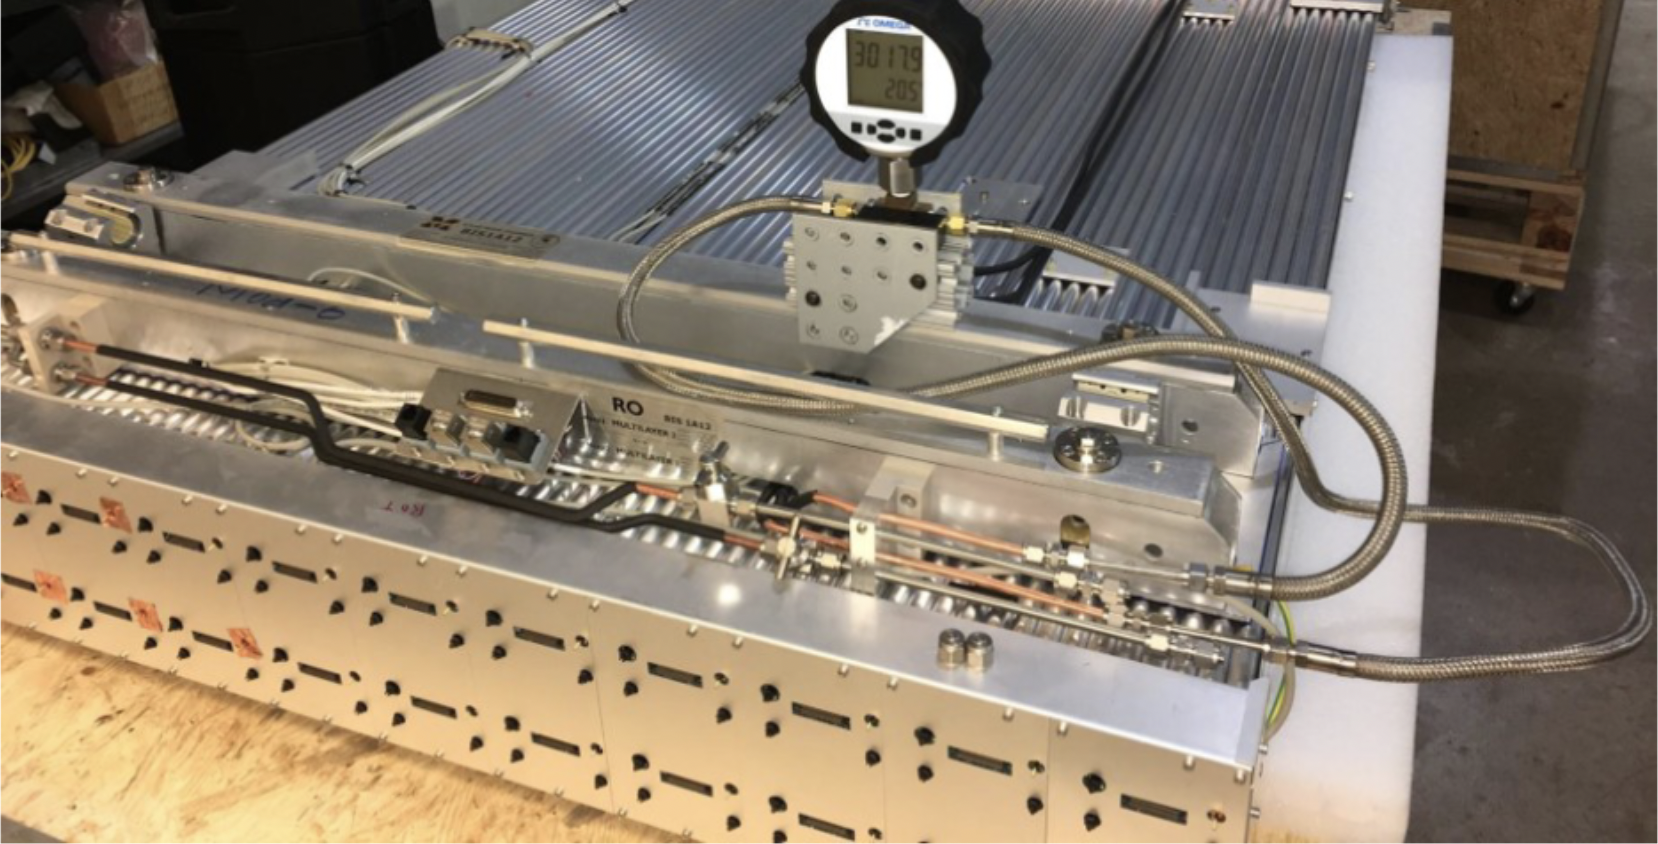
\includegraphics[width=0.5\pdfpagewidth]{PressureGauge.png}
		\end{figure}
		$$\Delta P_\text{corr}=P_f\frac{T_\text{ref}}{T_f}-P_i\frac{T_\text{ref}}{T_i}$$
	\end{frame}
	\begin{frame}{\hyperlinktarget{LeakRateTubes}{LeakRateTubesExtra}{Leak Rate Test - Tubes}}
		\begin{itemize}
			\item Ensures leak rate of individual tube is below 1E-5 mbar$\cdot$L/s.
			\item One tube at a time.
			\item Test takes $\sim2$ minutes.
			\item Tube is filled to 3 bar(a)
			\item Uses Leybold Quadro Phoenix Dry pump leak detector. 
		\end{itemize}
	\end{frame}
	\begin{frame}{\hyperlinktarget{TensionPhoto}{TensionExtra}{Tension - Extra}}
		\begin{itemize}
			\item Ensures tension of individual tube is between 325-380g.
			\item One tube at a time.
			\item Test takes $\sim30$ seconds.
			\item Tube is tested initially after construction, then tested 2 weeks after initial test. 
			\item Uses LabVIEW VI for signal generation and data collection.
		\end{itemize}
	\end{frame}
	\begin{frame}{\hyperlinktarget{DC}{DCExtra}{Dark Current - Extra}}
		\begin{itemize}
			\item Ensures noise rate of individual tube is below 2 nA.
			\item 48 tubes at a time.
			\item Test takes $\geq5$ hours.
			\item Tubes filled with 93:7 ArCO$_2$ at 3 bar(a), gas flowing at 1 SCFH. 
			\item Uses CAEN SY5527 power supply using CAEN GECO monitoring system.
		\end{itemize}
	\end{frame}
	\begin{frame}{Detailed UM Failure Rate}
		\begin{itemize}
			\item 19 Failed after construction during QA/QC tests. 
			\begin{itemize}
				\item 9 failed tension 
				\item 1 Leaked
				\item 1 had wire snap
				\item 1 had a crushed endpin.
				\item 1 had an electrical short
			\end{itemize}
			\item 44 raw tubes failed due to material deformities. (Bent, dent or deformities)
			\item 8 failed due to construction/mechanical errors that were seperate from normal testing.

		\end{itemize}
	\end{frame}
	\begin{frame}{DC Test - Extra}
		differences between tube test and chamber test
	\end{frame}
	\begin{frame}{Tension Test - Extra}
		Tension test is performed with LabVIEW.
	\end{frame}